\documentclass[1p]{elsarticle_modified}
%\bibliographystyle{elsarticle-num}

%\usepackage[colorlinks]{hyperref}
%\usepackage{abbrmath_seonhwa} %\Abb, \Ascr, \Acal ,\Abf, \Afrak
\usepackage{amsfonts}
\usepackage{amssymb}
\usepackage{amsmath}
\usepackage{amsthm}
\usepackage{scalefnt}
\usepackage{amsbsy}
\usepackage{kotex}
\usepackage{caption}
\usepackage{subfig}
\usepackage{color}
\usepackage{graphicx}
\usepackage{xcolor} %% white, black, red, green, blue, cyan, magenta, yellow
\usepackage{float}
\usepackage{setspace}
\usepackage{hyperref}

\usepackage{tikz}
\usetikzlibrary{arrows}

\usepackage{multirow}
\usepackage{array} % fixed length table
\usepackage{hhline}

%%%%%%%%%%%%%%%%%%%%%
\makeatletter
\renewcommand*\env@matrix[1][\arraystretch]{%
	\edef\arraystretch{#1}%
	\hskip -\arraycolsep
	\let\@ifnextchar\new@ifnextchar
	\array{*\c@MaxMatrixCols c}}
\makeatother %https://tex.stackexchange.com/questions/14071/how-can-i-increase-the-line-spacing-in-a-matrix
%%%%%%%%%%%%%%%

\usepackage[normalem]{ulem}

\newcommand{\msout}[1]{\ifmmode\text{\sout{\ensuremath{#1}}}\else\sout{#1}\fi}
%SOURCE: \msout is \stkout macro in https://tex.stackexchange.com/questions/20609/strikeout-in-math-mode

\newcommand{\cancel}[1]{
	\ifmmode
	{\color{red}\msout{#1}}
	\else
	{\color{red}\sout{#1}}
	\fi
}

\newcommand{\add}[1]{
	{\color{blue}\uwave{#1}}
}

\newcommand{\replace}[2]{
	\ifmmode
	{\color{red}\msout{#1}}{\color{blue}\uwave{#2}}
	\else
	{\color{red}\sout{#1}}{\color{blue}\uwave{#2}}
	\fi
}

\newcommand{\Sol}{\mathcal{S}} %segment
\newcommand{\D}{D} %diagram
\newcommand{\A}{\mathcal{A}} %arc


%%%%%%%%%%%%%%%%%%%%%%%%%%%%%5 test

\def\sl{\operatorname{\textup{SL}}(2,\Cbb)}
\def\psl{\operatorname{\textup{PSL}}(2,\Cbb)}
\def\quan{\mkern 1mu \triangleright \mkern 1mu}

\theoremstyle{definition}
\newtheorem{thm}{Theorem}[section]
\newtheorem{prop}[thm]{Proposition}
\newtheorem{lem}[thm]{Lemma}
\newtheorem{ques}[thm]{Question}
\newtheorem{cor}[thm]{Corollary}
\newtheorem{defn}[thm]{Definition}
\newtheorem{exam}[thm]{Example}
\newtheorem{rmk}[thm]{Remark}
\newtheorem{alg}[thm]{Algorithm}

\newcommand{\I}{\sqrt{-1}}
\begin{document}

%\begin{frontmatter}
%
%\title{Boundary parabolic representations of knots up to 8 crossings}
%
%%% Group authors per affiliation:
%\author{Yunhi Cho} 
%\address{Department of Mathematics, University of Seoul, Seoul, Korea}
%\ead{yhcho@uos.ac.kr}
%
%
%\author{Seonhwa Kim} %\fnref{s_kim}}
%\address{Center for Geometry and Physics, Institute for Basic Science, Pohang, 37673, Korea}
%\ead{ryeona17@ibs.re.kr}
%
%\author{Hyuk Kim}
%\address{Department of Mathematical Sciences, Seoul National University, Seoul 08826, Korea}
%\ead{hyukkim@snu.ac.kr}
%
%\author{Seokbeom Yoon}
%\address{Department of Mathematical Sciences, Seoul National University, Seoul, 08826,  Korea}
%\ead{sbyoon15@snu.ac.kr}
%
%\begin{abstract}
%We find all boundary parabolic representation of knots up to 8 crossings.
%
%\end{abstract}
%\begin{keyword}
%    \MSC[2010] 57M25 
%\end{keyword}
%
%\end{frontmatter}

%\linenumbers
%\tableofcontents
%
\newcommand\colored[1]{\textcolor{white}{\rule[-0.35ex]{0.8em}{1.4ex}}\kern-0.8em\color{red} #1}%
%\newcommand\colored[1]{\textcolor{white}{ #1}\kern-2.17ex	\textcolor{white}{ #1}\kern-1.81ex	\textcolor{white}{ #1}\kern-2.15ex\color{red}#1	}

{\Large $\underline{12a_{0860}~(K12a_{0860})}$}

\setlength{\tabcolsep}{10pt}
\renewcommand{\arraystretch}{1.6}
\vspace{1cm}\begin{tabular}{m{100pt}>{\centering\arraybackslash}m{274pt}}
\multirow{5}{120pt}{
	\centering
	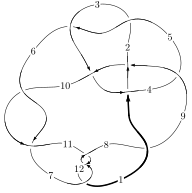
\includegraphics[width=112pt]{../../../GIT/diagram.site/Diagrams/png/1661_12a_0860.png}\\
\ \ \ A knot diagram\footnotemark}&
\allowdisplaybreaks
\textbf{Linearized knot diagam} \\
\cline{2-2}
 &
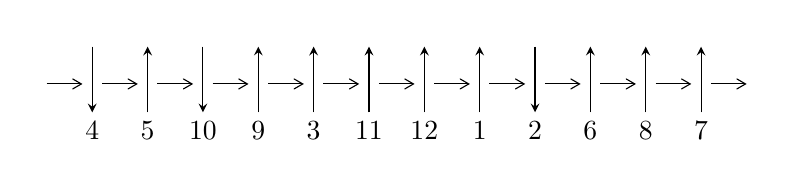
\begin{tikzpicture}[x=20pt, y=17pt]
	% nodes
	\node (C0) at (0, 0) {};
	\node (C1) at (1, 0) {};
	\node (C1U) at (1, +1) {};
	\node (C1D) at (1, -1) {4};

	\node (C2) at (2, 0) {};
	\node (C2U) at (2, +1) {};
	\node (C2D) at (2, -1) {5};

	\node (C3) at (3, 0) {};
	\node (C3U) at (3, +1) {};
	\node (C3D) at (3, -1) {10};

	\node (C4) at (4, 0) {};
	\node (C4U) at (4, +1) {};
	\node (C4D) at (4, -1) {9};

	\node (C5) at (5, 0) {};
	\node (C5U) at (5, +1) {};
	\node (C5D) at (5, -1) {3};

	\node (C6) at (6, 0) {};
	\node (C6U) at (6, +1) {};
	\node (C6D) at (6, -1) {11};

	\node (C7) at (7, 0) {};
	\node (C7U) at (7, +1) {};
	\node (C7D) at (7, -1) {12};

	\node (C8) at (8, 0) {};
	\node (C8U) at (8, +1) {};
	\node (C8D) at (8, -1) {1};

	\node (C9) at (9, 0) {};
	\node (C9U) at (9, +1) {};
	\node (C9D) at (9, -1) {2};

	\node (C10) at (10, 0) {};
	\node (C10U) at (10, +1) {};
	\node (C10D) at (10, -1) {6};

	\node (C11) at (11, 0) {};
	\node (C11U) at (11, +1) {};
	\node (C11D) at (11, -1) {8};

	\node (C12) at (12, 0) {};
	\node (C12U) at (12, +1) {};
	\node (C12D) at (12, -1) {7};
	\node (C13) at (13, 0) {};

	% arrows
	\draw[->,>={angle 60}]
	(C0) edge (C1) (C1) edge (C2) (C2) edge (C3) (C3) edge (C4) (C4) edge (C5) (C5) edge (C6) (C6) edge (C7) (C7) edge (C8) (C8) edge (C9) (C9) edge (C10) (C10) edge (C11) (C11) edge (C12) (C12) edge (C13) ;	\draw[->,>=stealth]
	(C1U) edge (C1D) (C2D) edge (C2U) (C3U) edge (C3D) (C4D) edge (C4U) (C5D) edge (C5U) (C6D) edge (C6U) (C7D) edge (C7U) (C8D) edge (C8U) (C9U) edge (C9D) (C10D) edge (C10U) (C11D) edge (C11U) (C12D) edge (C12U) ;
	\end{tikzpicture} \\
\hhline{~~} \\& 
\textbf{Solving Sequence} \\ \cline{2-2} 
 &
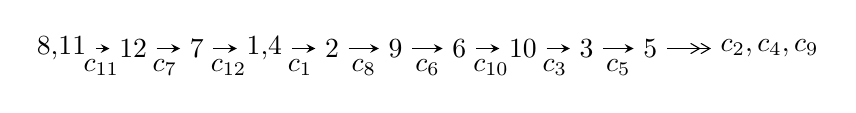
\begin{tikzpicture}[x=23pt, y=7pt]
	% node
	\node (A0) at (-1/8, 0) {8,11};
	\node (A1) at (1, 0) {12};
	\node (A2) at (2, 0) {7};
	\node (A3) at (49/16, 0) {1,4};
	\node (A4) at (33/8, 0) {2};
	\node (A5) at (41/8, 0) {9};
	\node (A6) at (49/8, 0) {6};
	\node (A7) at (57/8, 0) {10};
	\node (A8) at (65/8, 0) {3};
	\node (A9) at (73/8, 0) {5};
	\node (C1) at (1/2, -1) {$c_{11}$};
	\node (C2) at (3/2, -1) {$c_{7}$};
	\node (C3) at (5/2, -1) {$c_{12}$};
	\node (C4) at (29/8, -1) {$c_{1}$};
	\node (C5) at (37/8, -1) {$c_{8}$};
	\node (C6) at (45/8, -1) {$c_{6}$};
	\node (C7) at (53/8, -1) {$c_{10}$};
	\node (C8) at (61/8, -1) {$c_{3}$};
	\node (C9) at (69/8, -1) {$c_{5}$};
	\node (A10) at (11, 0) {$c_{2},c_{4},c_{9}$};

	% edge
	\draw[->,>=stealth]	
	(A0) edge (A1) (A1) edge (A2) (A2) edge (A3) (A3) edge (A4) (A4) edge (A5) (A5) edge (A6) (A6) edge (A7) (A7) edge (A8) (A8) edge (A9) ;
	\draw[->>,>={angle 60}]	
	(A9) edge (A10);
\end{tikzpicture} \\ 

\end{tabular} \\

\footnotetext{
The image of knot diagram is generated by the software ``\textbf{Draw programme}" developed by Andrew Bartholomew(\url{http://www.layer8.co.uk/maths/draw/index.htm\#Running-draw}), where we modified some parts for our purpose(\url{https://github.com/CATsTAILs/LinksPainter}).
}\phantom \\ \newline 
\centering \textbf{Ideals for irreducible components\footnotemark of $X_{\text{par}}$} 
 
\begin{align*}
I^u_{1}&=\langle 
-5.29007\times10^{24} u^{76}+1.01626\times10^{25} u^{75}+\cdots+1.55594\times10^{24} b+8.02867\times10^{24},\\
\phantom{I^u_{1}}&\phantom{= \langle  }8.96223\times10^{24} u^{76}-1.26342\times10^{25} u^{75}+\cdots+1.55594\times10^{24} a-1.05097\times10^{25},\;u^{77}-2 u^{76}+\cdots-7 u+1\rangle \\
I^u_{2}&=\langle 
u^2+b+1,\;- u^2+a-2,\;u^3- u^2+2 u-1\rangle \\
\\
\end{align*}
\raggedright * 2 irreducible components of $\dim_{\mathbb{C}}=0$, with total 80 representations.\\
\footnotetext{All coefficients of polynomials are rational numbers. But the coefficients are sometimes approximated in decimal forms when there is not enough margin.}
\newpage
\renewcommand{\arraystretch}{1}
\centering \section*{I. $I^u_{1}= \langle -5.29\times10^{24} u^{76}+1.02\times10^{25} u^{75}+\cdots+1.56\times10^{24} b+8.03\times10^{24},\;8.96\times10^{24} u^{76}-1.26\times10^{25} u^{75}+\cdots+1.56\times10^{24} a-1.05\times10^{25},\;u^{77}-2 u^{76}+\cdots-7 u+1 \rangle$}
\flushleft \textbf{(i) Arc colorings}\\
\begin{tabular}{m{7pt} m{180pt} m{7pt} m{180pt} }
\flushright $a_{8}=$&$\begin{pmatrix}0\\u\end{pmatrix}$ \\
\flushright $a_{11}=$&$\begin{pmatrix}1\\0\end{pmatrix}$ \\
\flushright $a_{12}=$&$\begin{pmatrix}1\\- u^2\end{pmatrix}$ \\
\flushright $a_{7}=$&$\begin{pmatrix}- u\\u^3+u\end{pmatrix}$ \\
\flushright $a_{1}=$&$\begin{pmatrix}u^2+1\\- u^4-2 u^2\end{pmatrix}$ \\
\flushright $a_{4}=$&$\begin{pmatrix}-5.76000 u^{76}+8.11999 u^{75}+\cdots-49.9977 u+6.75457\\3.39991 u^{76}-6.53146 u^{75}+\cdots+29.1654 u-5.16000\end{pmatrix}$ \\
\flushright $a_{2}=$&$\begin{pmatrix}0.200000 u^{76}+0.0000233782 u^{75}+\cdots-1.10414 u-0.722387\\-0.400023 u^{76}-0.0418941 u^{75}+\cdots-0.677613 u+0.200000\end{pmatrix}$ \\
\flushright $a_{9}=$&$\begin{pmatrix}u^5+2 u^3+u\\- u^7-3 u^5-2 u^3+u\end{pmatrix}$ \\
\flushright $a_{6}=$&$\begin{pmatrix}- u^3-2 u\\u^3+u\end{pmatrix}$ \\
\flushright $a_{10}=$&$\begin{pmatrix}- u^6-3 u^4-2 u^2+1\\u^6+2 u^4+u^2\end{pmatrix}$ \\
\flushright $a_{3}=$&$\begin{pmatrix}-4.16000 u^{76}+4.92014 u^{75}+\cdots-30.5063 u+3.54293\\3.60000 u^{76}-6.98916 u^{75}+\cdots+37.6171 u-6.96000\end{pmatrix}$ \\
\flushright $a_{5}=$&$\begin{pmatrix}-3.96000 u^{76}+4.71990 u^{75}+\cdots-32.2944 u+3.21217\\3.40001 u^{76}-6.65993 u^{75}+\cdots+37.1478 u-6.76000\end{pmatrix}$\\&\end{tabular}
\flushleft \textbf{(ii) Obstruction class $= -1$}\\~\\
\flushleft \textbf{(iii) Cusp Shapes $= \frac{39428653274113013343690898}{1555942872114780833899609} u^{76}-\frac{62426554058064260098232498}{1555942872114780833899609} u^{75}+\cdots+\frac{513166216142495611295460359}{1555942872114780833899609} u-\frac{100110429527755677393611749}{1555942872114780833899609}$}\\~\\
\newpage\renewcommand{\arraystretch}{1}
\flushleft \textbf{(iv) u-Polynomials at the component}\newline \\
\begin{tabular}{m{50pt}|m{274pt}}
Crossings & \hspace{64pt}u-Polynomials at each crossing \\
\hline $$\begin{aligned}c_{1}\end{aligned}$$&$\begin{aligned}
&u^{77}-13 u^{76}+\cdots+20 u+8
\end{aligned}$\\
\hline $$\begin{aligned}c_{2},c_{5}\end{aligned}$$&$\begin{aligned}
&u^{77}+4 u^{76}+\cdots-14 u+1
\end{aligned}$\\
\hline $$\begin{aligned}c_{3}\end{aligned}$$&$\begin{aligned}
&u^{77}+u^{76}+\cdots+887410 u+302321
\end{aligned}$\\
\hline $$\begin{aligned}c_{4}\end{aligned}$$&$\begin{aligned}
&u^{77}+3 u^{76}+\cdots-1548 u+181
\end{aligned}$\\
\hline $$\begin{aligned}c_{6},c_{8},c_{10}\end{aligned}$$&$\begin{aligned}
&u^{77}+2 u^{76}+\cdots-147 u+17
\end{aligned}$\\
\hline $$\begin{aligned}c_{7},c_{11},c_{12}\end{aligned}$$&$\begin{aligned}
&u^{77}-2 u^{76}+\cdots-7 u+1
\end{aligned}$\\
\hline $$\begin{aligned}c_{9}\end{aligned}$$&$\begin{aligned}
&u^{77}-2 u^{76}+\cdots- u+1
\end{aligned}$\\
\hline
\end{tabular}\\~\\
\newpage\renewcommand{\arraystretch}{1}
\flushleft \textbf{(v) Riley Polynomials at the component}\newline \\
\begin{tabular}{m{50pt}|m{274pt}}
Crossings & \hspace{64pt}Riley Polynomials at each crossing \\
\hline $$\begin{aligned}c_{1}\end{aligned}$$&$\begin{aligned}
&y^{77}+21 y^{76}+\cdots-432 y-64
\end{aligned}$\\
\hline $$\begin{aligned}c_{2},c_{5}\end{aligned}$$&$\begin{aligned}
&y^{77}-62 y^{76}+\cdots+26 y-1
\end{aligned}$\\
\hline $$\begin{aligned}c_{3}\end{aligned}$$&$\begin{aligned}
&y^{77}-33 y^{76}+\cdots-1941705110116 y-91397987041
\end{aligned}$\\
\hline $$\begin{aligned}c_{4}\end{aligned}$$&$\begin{aligned}
&y^{77}-101 y^{76}+\cdots+3284652 y-32761
\end{aligned}$\\
\hline $$\begin{aligned}c_{6},c_{8},c_{10}\end{aligned}$$&$\begin{aligned}
&y^{77}-84 y^{76}+\cdots-4639 y-289
\end{aligned}$\\
\hline $$\begin{aligned}c_{7},c_{11},c_{12}\end{aligned}$$&$\begin{aligned}
&y^{77}+60 y^{76}+\cdots+y-1
\end{aligned}$\\
\hline $$\begin{aligned}c_{9}\end{aligned}$$&$\begin{aligned}
&y^{77}+12 y^{76}+\cdots+y-1
\end{aligned}$\\
\hline
\end{tabular}\\~\\
\newpage\flushleft \textbf{(vi) Complex Volumes and Cusp Shapes}
$$\begin{array}{c|c|c}  
\text{Solutions to }I^u_{1}& \I (\text{vol} + \sqrt{-1}CS) & \text{Cusp shape}\\
 \hline 
\begin{aligned}
u &= -0.913802 + 0.063108 I \\
a &= \phantom{-}0.33472 - 1.92033 I \\
b &= -0.27119 + 1.94599 I\end{aligned}
 & \phantom{-}13.03970 - 3.23619 I & \phantom{-}15.5734 + 0. I\phantom{ +0.000000I} \\ \hline\begin{aligned}
u &= -0.913802 - 0.063108 I \\
a &= \phantom{-}0.33472 + 1.92033 I \\
b &= -0.27119 - 1.94599 I\end{aligned}
 & \phantom{-}13.03970 + 3.23619 I & \phantom{-}15.5734 + 0. I\phantom{ +0.000000I} \\ \hline\begin{aligned}
u &= \phantom{-}0.906595 + 0.055280 I \\
a &= \phantom{-}0.34629 - 3.14143 I \\
b &= -0.32424 + 3.20304 I\end{aligned}
 & \phantom{-}13.6932 + 11.6268 I & \phantom{-}13.0485 - 6.1237 I \\ \hline\begin{aligned}
u &= \phantom{-}0.906595 - 0.055280 I \\
a &= \phantom{-}0.34629 + 3.14143 I \\
b &= -0.32424 - 3.20304 I\end{aligned}
 & \phantom{-}13.6932 - 11.6268 I & \phantom{-}13.0485 + 6.1237 I \\ \hline\begin{aligned}
u &= -0.326996 + 0.842532 I \\
a &= -0.541376 + 0.646495 I \\
b &= \phantom{-}0.402390 - 0.782201 I\end{aligned}
 & \phantom{-}3.66083 + 4.79876 I & \phantom{-0.000000 } 0 \\ \hline\begin{aligned}
u &= -0.326996 - 0.842532 I \\
a &= -0.541376 - 0.646495 I \\
b &= \phantom{-}0.402390 + 0.782201 I\end{aligned}
 & \phantom{-}3.66083 - 4.79876 I & \phantom{-0.000000 } 0 \\ \hline\begin{aligned}
u &= \phantom{-}0.894206 + 0.008927 I \\
a &= \phantom{-}1.91536 + 2.58709 I \\
b &= -1.44994 - 2.51862 I\end{aligned}
 & \phantom{-}12.52080 + 2.21530 I & \phantom{-}17.1121 - 3.0542 I \\ \hline\begin{aligned}
u &= \phantom{-}0.894206 - 0.008927 I \\
a &= \phantom{-}1.91536 - 2.58709 I \\
b &= -1.44994 + 2.51862 I\end{aligned}
 & \phantom{-}12.52080 - 2.21530 I & \phantom{-}17.1121 + 3.0542 I \\ \hline\begin{aligned}
u &= \phantom{-}0.887210 + 0.029674 I \\
a &= -0.78127 + 3.57061 I \\
b &= \phantom{-}0.65963 - 3.44289 I\end{aligned}
 & \phantom{-}8.27458 + 5.48443 I & \phantom{-}11.67244 - 5.84044 I \\ \hline\begin{aligned}
u &= \phantom{-}0.887210 - 0.029674 I \\
a &= -0.78127 - 3.57061 I \\
b &= \phantom{-}0.65963 + 3.44289 I\end{aligned}
 & \phantom{-}8.27458 - 5.48443 I & \phantom{-}11.67244 + 5.84044 I\\
 \hline 
 \end{array}$$\newpage$$\begin{array}{c|c|c}  
\text{Solutions to }I^u_{1}& \I (\text{vol} + \sqrt{-1}CS) & \text{Cusp shape}\\
 \hline 
\begin{aligned}
u &= -0.054607 + 1.112520 I \\
a &= \phantom{-}0.513405 - 1.069200 I \\
b &= -0.660143 + 0.296254 I\end{aligned}
 & -1.43943 + 1.45452 I & \phantom{-0.000000 } 0 \\ \hline\begin{aligned}
u &= -0.054607 - 1.112520 I \\
a &= \phantom{-}0.513405 + 1.069200 I \\
b &= -0.660143 - 0.296254 I\end{aligned}
 & -1.43943 - 1.45452 I & \phantom{-0.000000 } 0 \\ \hline\begin{aligned}
u &= -0.882807\phantom{ +0.000000I} \\
a &= \phantom{-}2.61824\phantom{ +0.000000I} \\
b &= -3.54585\phantom{ +0.000000I}\end{aligned}
 & \phantom{-}9.90045\phantom{ +0.000000I} & -3.11330\phantom{ +0.000000I} \\ \hline\begin{aligned}
u &= -0.874751 + 0.019237 I \\
a &= -0.76012 + 2.37591 I \\
b &= \phantom{-}0.95744 - 2.48019 I\end{aligned}
 & \phantom{-}7.97257 - 1.22260 I & \phantom{-}10.90582 - 1.45578 I \\ \hline\begin{aligned}
u &= -0.874751 - 0.019237 I \\
a &= -0.76012 - 2.37591 I \\
b &= \phantom{-}0.95744 + 2.48019 I\end{aligned}
 & \phantom{-}7.97257 + 1.22260 I & \phantom{-}10.90582 + 1.45578 I \\ \hline\begin{aligned}
u &= \phantom{-}0.361283 + 0.751844 I \\
a &= -0.295918 + 0.495393 I \\
b &= \phantom{-}0.171946 - 0.640949 I\end{aligned}
 & \phantom{-}3.46003 + 4.32392 I & \phantom{-}11.42298 - 6.33256 I \\ \hline\begin{aligned}
u &= \phantom{-}0.361283 - 0.751844 I \\
a &= -0.295918 - 0.495393 I \\
b &= \phantom{-}0.171946 + 0.640949 I\end{aligned}
 & \phantom{-}3.46003 - 4.32392 I & \phantom{-}11.42298 + 6.33256 I \\ \hline\begin{aligned}
u &= -0.183088 + 1.165940 I \\
a &= -0.266992 - 0.369562 I \\
b &= -1.37755 + 1.07744 I\end{aligned}
 & \phantom{-}1.26375 - 1.05598 I & \phantom{-0.000000 } 0 \\ \hline\begin{aligned}
u &= -0.183088 - 1.165940 I \\
a &= -0.266992 + 0.369562 I \\
b &= -1.37755 - 1.07744 I\end{aligned}
 & \phantom{-}1.26375 + 1.05598 I & \phantom{-0.000000 } 0 \\ \hline\begin{aligned}
u &= \phantom{-}0.092580 + 1.209120 I \\
a &= \phantom{-}0.10678 - 1.57343 I \\
b &= -1.35466 + 0.92333 I\end{aligned}
 & -1.84582 + 1.52815 I & \phantom{-0.000000 } 0\\
 \hline 
 \end{array}$$\newpage$$\begin{array}{c|c|c}  
\text{Solutions to }I^u_{1}& \I (\text{vol} + \sqrt{-1}CS) & \text{Cusp shape}\\
 \hline 
\begin{aligned}
u &= \phantom{-}0.092580 - 1.209120 I \\
a &= \phantom{-}0.10678 + 1.57343 I \\
b &= -1.35466 - 0.92333 I\end{aligned}
 & -1.84582 - 1.52815 I & \phantom{-0.000000 } 0 \\ \hline\begin{aligned}
u &= \phantom{-}0.161416 + 1.229950 I \\
a &= \phantom{-}0.15681 + 2.49802 I \\
b &= \phantom{-}3.50115 - 1.48373 I\end{aligned}
 & -1.14368 + 2.23292 I & \phantom{-0.000000 } 0 \\ \hline\begin{aligned}
u &= \phantom{-}0.161416 - 1.229950 I \\
a &= \phantom{-}0.15681 - 2.49802 I \\
b &= \phantom{-}3.50115 + 1.48373 I\end{aligned}
 & -1.14368 - 2.23292 I & \phantom{-0.000000 } 0 \\ \hline\begin{aligned}
u &= -0.210827 + 1.234980 I \\
a &= -0.754554 + 0.782417 I \\
b &= -0.430198 + 0.502926 I\end{aligned}
 & \phantom{-}0.54834 - 4.47323 I & \phantom{-0.000000 } 0 \\ \hline\begin{aligned}
u &= -0.210827 - 1.234980 I \\
a &= -0.754554 - 0.782417 I \\
b &= -0.430198 - 0.502926 I\end{aligned}
 & \phantom{-}0.54834 + 4.47323 I & \phantom{-0.000000 } 0 \\ \hline\begin{aligned}
u &= \phantom{-}0.658448 + 0.323972 I \\
a &= \phantom{-}0.751995 + 0.291567 I \\
b &= \phantom{-}0.029394 - 0.146081 I\end{aligned}
 & \phantom{-}4.80945 - 0.45159 I & \phantom{-}15.7916 + 0.4639 I \\ \hline\begin{aligned}
u &= \phantom{-}0.658448 - 0.323972 I \\
a &= \phantom{-}0.751995 - 0.291567 I \\
b &= \phantom{-}0.029394 + 0.146081 I\end{aligned}
 & \phantom{-}4.80945 + 0.45159 I & \phantom{-}15.7916 - 0.4639 I \\ \hline\begin{aligned}
u &= \phantom{-}0.150237 + 1.273730 I \\
a &= \phantom{-}0.526714 + 0.048722 I \\
b &= -0.812204 - 0.549214 I\end{aligned}
 & -3.21431 + 2.39962 I & \phantom{-0.000000 } 0 \\ \hline\begin{aligned}
u &= \phantom{-}0.150237 - 1.273730 I \\
a &= \phantom{-}0.526714 - 0.048722 I \\
b &= -0.812204 + 0.549214 I\end{aligned}
 & -3.21431 - 2.39962 I & \phantom{-0.000000 } 0 \\ \hline\begin{aligned}
u &= -0.658985 + 0.265213 I \\
a &= -0.49122 + 1.57510 I \\
b &= -0.125247 - 0.445150 I\end{aligned}
 & \phantom{-}5.38906 - 8.57192 I & \phantom{-}11.9706 + 8.1913 I\\
 \hline 
 \end{array}$$\newpage$$\begin{array}{c|c|c}  
\text{Solutions to }I^u_{1}& \I (\text{vol} + \sqrt{-1}CS) & \text{Cusp shape}\\
 \hline 
\begin{aligned}
u &= -0.658985 - 0.265213 I \\
a &= -0.49122 - 1.57510 I \\
b &= -0.125247 + 0.445150 I\end{aligned}
 & \phantom{-}5.38906 + 8.57192 I & \phantom{-}11.9706 - 8.1913 I \\ \hline\begin{aligned}
u &= \phantom{-}0.698912\phantom{ +0.000000I} \\
a &= -1.05888\phantom{ +0.000000I} \\
b &= \phantom{-}0.453650\phantom{ +0.000000I}\end{aligned}
 & \phantom{-}1.62149\phantom{ +0.000000I} & \phantom{-}4.73710\phantom{ +0.000000I} \\ \hline\begin{aligned}
u &= -0.028016 + 1.301540 I \\
a &= \phantom{-}0.256976 + 0.051421 I \\
b &= \phantom{-}1.053210 - 0.861329 I\end{aligned}
 & -5.86592 + 1.11778 I & \phantom{-0.000000 } 0 \\ \hline\begin{aligned}
u &= -0.028016 - 1.301540 I \\
a &= \phantom{-}0.256976 - 0.051421 I \\
b &= \phantom{-}1.053210 + 0.861329 I\end{aligned}
 & -5.86592 - 1.11778 I & \phantom{-0.000000 } 0 \\ \hline\begin{aligned}
u &= \phantom{-}0.289500 + 1.270280 I \\
a &= \phantom{-}0.234588 - 0.583710 I \\
b &= -0.548186 + 0.321533 I\end{aligned}
 & -2.33279 + 3.56920 I & \phantom{-0.000000 } 0 \\ \hline\begin{aligned}
u &= \phantom{-}0.289500 - 1.270280 I \\
a &= \phantom{-}0.234588 + 0.583710 I \\
b &= -0.548186 - 0.321533 I\end{aligned}
 & -2.33279 - 3.56920 I & \phantom{-0.000000 } 0 \\ \hline\begin{aligned}
u &= -0.198314 + 1.296690 I \\
a &= -0.502123 + 0.738377 I \\
b &= \phantom{-}0.980901 - 0.670423 I\end{aligned}
 & -3.85925 - 6.47132 I & \phantom{-0.000000 } 0 \\ \hline\begin{aligned}
u &= -0.198314 - 1.296690 I \\
a &= -0.502123 - 0.738377 I \\
b &= \phantom{-}0.980901 + 0.670423 I\end{aligned}
 & -3.85925 + 6.47132 I & \phantom{-0.000000 } 0 \\ \hline\begin{aligned}
u &= -0.462815 + 1.228630 I \\
a &= \phantom{-}1.063350 - 0.751492 I \\
b &= \phantom{-}0.73021 + 1.61220 I\end{aligned}
 & \phantom{-}9.44703 - 1.66736 I & \phantom{-0.000000 } 0 \\ \hline\begin{aligned}
u &= -0.462815 - 1.228630 I \\
a &= \phantom{-}1.063350 + 0.751492 I \\
b &= \phantom{-}0.73021 - 1.61220 I\end{aligned}
 & \phantom{-}9.44703 + 1.66736 I & \phantom{-0.000000 } 0\\
 \hline 
 \end{array}$$\newpage$$\begin{array}{c|c|c}  
\text{Solutions to }I^u_{1}& \I (\text{vol} + \sqrt{-1}CS) & \text{Cusp shape}\\
 \hline 
\begin{aligned}
u &= \phantom{-}0.453502 + 1.234510 I \\
a &= -2.00885 - 0.56842 I \\
b &= -0.42347 + 2.73870 I\end{aligned}
 & \phantom{-}10.05520 - 6.77668 I & \phantom{-0.000000 } 0 \\ \hline\begin{aligned}
u &= \phantom{-}0.453502 - 1.234510 I \\
a &= -2.00885 + 0.56842 I \\
b &= -0.42347 - 2.73870 I\end{aligned}
 & \phantom{-}10.05520 + 6.77668 I & \phantom{-0.000000 } 0 \\ \hline\begin{aligned}
u &= \phantom{-}0.426332 + 1.253220 I \\
a &= \phantom{-}2.34854 + 0.48663 I \\
b &= \phantom{-}0.11887 - 3.15154 I\end{aligned}
 & \phantom{-}4.48799 - 0.78739 I & \phantom{-0.000000 } 0 \\ \hline\begin{aligned}
u &= \phantom{-}0.426332 - 1.253220 I \\
a &= \phantom{-}2.34854 - 0.48663 I \\
b &= \phantom{-}0.11887 + 3.15154 I\end{aligned}
 & \phantom{-}4.48799 + 0.78739 I & \phantom{-0.000000 } 0 \\ \hline\begin{aligned}
u &= -0.413163 + 1.260620 I \\
a &= -1.26088 + 1.13233 I \\
b &= -1.70921 - 1.82672 I\end{aligned}
 & \phantom{-}4.12598 - 3.38895 I & \phantom{-0.000000 } 0 \\ \hline\begin{aligned}
u &= -0.413163 - 1.260620 I \\
a &= -1.26088 - 1.13233 I \\
b &= -1.70921 + 1.82672 I\end{aligned}
 & \phantom{-}4.12598 + 3.38895 I & \phantom{-0.000000 } 0 \\ \hline\begin{aligned}
u &= \phantom{-}0.427750 + 1.273090 I \\
a &= \phantom{-}0.95805 + 1.80831 I \\
b &= \phantom{-}1.99298 - 2.44923 I\end{aligned}
 & \phantom{-}8.59850 + 2.51088 I & \phantom{-0.000000 } 0 \\ \hline\begin{aligned}
u &= \phantom{-}0.427750 - 1.273090 I \\
a &= \phantom{-}0.95805 - 1.80831 I \\
b &= \phantom{-}1.99298 + 2.44923 I\end{aligned}
 & \phantom{-}8.59850 - 2.51088 I & \phantom{-0.000000 } 0 \\ \hline\begin{aligned}
u &= -0.416478 + 1.278250 I \\
a &= -0.43242 - 1.68397 I \\
b &= \phantom{-}3.25434 - 1.51855 I\end{aligned}
 & \phantom{-}5.93001 - 4.65047 I & \phantom{-0.000000 } 0 \\ \hline\begin{aligned}
u &= -0.416478 - 1.278250 I \\
a &= -0.43242 + 1.68397 I \\
b &= \phantom{-}3.25434 + 1.51855 I\end{aligned}
 & \phantom{-}5.93001 + 4.65047 I & \phantom{-0.000000 } 0\\
 \hline 
 \end{array}$$\newpage$$\begin{array}{c|c|c}  
\text{Solutions to }I^u_{1}& \I (\text{vol} + \sqrt{-1}CS) & \text{Cusp shape}\\
 \hline 
\begin{aligned}
u &= -0.406803 + 1.291700 I \\
a &= \phantom{-}1.52766 - 0.20602 I \\
b &= -0.06857 + 2.76086 I\end{aligned}
 & \phantom{-}3.89118 - 5.81428 I & \phantom{-0.000000 } 0 \\ \hline\begin{aligned}
u &= -0.406803 - 1.291700 I \\
a &= \phantom{-}1.52766 + 0.20602 I \\
b &= -0.06857 - 2.76086 I\end{aligned}
 & \phantom{-}3.89118 + 5.81428 I & \phantom{-0.000000 } 0 \\ \hline\begin{aligned}
u &= \phantom{-}0.423725 + 1.287430 I \\
a &= -2.12946 + 0.38318 I \\
b &= \phantom{-}0.97652 + 2.37850 I\end{aligned}
 & \phantom{-}8.49017 + 6.92911 I & \phantom{-0.000000 } 0 \\ \hline\begin{aligned}
u &= \phantom{-}0.423725 - 1.287430 I \\
a &= -2.12946 - 0.38318 I \\
b &= \phantom{-}0.97652 - 2.37850 I\end{aligned}
 & \phantom{-}8.49017 - 6.92911 I & \phantom{-0.000000 } 0 \\ \hline\begin{aligned}
u &= \phantom{-}0.414262 + 1.301330 I \\
a &= -1.85647 - 1.47317 I \\
b &= -1.45440 + 3.42200 I\end{aligned}
 & \phantom{-}4.12642 + 10.14420 I & \phantom{-0.000000 } 0 \\ \hline\begin{aligned}
u &= \phantom{-}0.414262 - 1.301330 I \\
a &= -1.85647 + 1.47317 I \\
b &= -1.45440 - 3.42200 I\end{aligned}
 & \phantom{-}4.12642 - 10.14420 I & \phantom{-0.000000 } 0 \\ \hline\begin{aligned}
u &= -0.235156 + 1.346920 I \\
a &= \phantom{-}0.733057 - 0.616515 I \\
b &= -0.596383 + 0.773379 I\end{aligned}
 & \phantom{-}0.32118 - 11.71550 I & \phantom{-0.000000 } 0 \\ \hline\begin{aligned}
u &= -0.235156 - 1.346920 I \\
a &= \phantom{-}0.733057 + 0.616515 I \\
b &= -0.596383 - 0.773379 I\end{aligned}
 & \phantom{-}0.32118 + 11.71550 I & \phantom{-0.000000 } 0 \\ \hline\begin{aligned}
u &= \phantom{-}0.026010 + 1.380640 I \\
a &= \phantom{-}0.0205117 + 0.0989125 I \\
b &= -0.763915 + 0.702888 I\end{aligned}
 & -3.00730 + 4.91043 I & \phantom{-0.000000 } 0 \\ \hline\begin{aligned}
u &= \phantom{-}0.026010 - 1.380640 I \\
a &= \phantom{-}0.0205117 - 0.0989125 I \\
b &= -0.763915 - 0.702888 I\end{aligned}
 & -3.00730 - 4.91043 I & \phantom{-0.000000 } 0\\
 \hline 
 \end{array}$$\newpage$$\begin{array}{c|c|c}  
\text{Solutions to }I^u_{1}& \I (\text{vol} + \sqrt{-1}CS) & \text{Cusp shape}\\
 \hline 
\begin{aligned}
u &= \phantom{-}0.421371 + 1.322560 I \\
a &= \phantom{-}1.76986 + 1.12258 I \\
b &= \phantom{-}1.11872 - 3.28566 I\end{aligned}
 & \phantom{-}9.3880 + 16.3776 I & \phantom{-0.000000 } 0 \\ \hline\begin{aligned}
u &= \phantom{-}0.421371 - 1.322560 I \\
a &= \phantom{-}1.76986 - 1.12258 I \\
b &= \phantom{-}1.11872 + 3.28566 I\end{aligned}
 & \phantom{-}9.3880 - 16.3776 I & \phantom{-0.000000 } 0 \\ \hline\begin{aligned}
u &= -0.424789 + 1.329390 I \\
a &= -1.208660 + 0.425059 I \\
b &= -0.22264 - 1.99964 I\end{aligned}
 & \phantom{-}8.68598 - 8.02392 I & \phantom{-0.000000 } 0 \\ \hline\begin{aligned}
u &= -0.424789 - 1.329390 I \\
a &= -1.208660 - 0.425059 I \\
b &= -0.22264 + 1.99964 I\end{aligned}
 & \phantom{-}8.68598 + 8.02392 I & \phantom{-0.000000 } 0 \\ \hline\begin{aligned}
u &= \phantom{-}0.220478 + 1.386360 I \\
a &= -0.368808 + 0.007896 I \\
b &= \phantom{-}0.224428 - 0.133536 I\end{aligned}
 & -0.63581 + 2.62873 I & \phantom{-0.000000 } 0 \\ \hline\begin{aligned}
u &= \phantom{-}0.220478 - 1.386360 I \\
a &= -0.368808 - 0.007896 I \\
b &= \phantom{-}0.224428 + 0.133536 I\end{aligned}
 & -0.63581 - 2.62873 I & \phantom{-0.000000 } 0 \\ \hline\begin{aligned}
u &= -0.539636 + 0.187893 I \\
a &= \phantom{-}0.42741 - 1.76367 I \\
b &= -0.1137720 + 0.0518232 I\end{aligned}
 & \phantom{-}0.70764 - 3.84105 I & \phantom{-}9.38498 + 8.87377 I \\ \hline\begin{aligned}
u &= -0.539636 - 0.187893 I \\
a &= \phantom{-}0.42741 + 1.76367 I \\
b &= -0.1137720 - 0.0518232 I\end{aligned}
 & \phantom{-}0.70764 + 3.84105 I & \phantom{-}9.38498 - 8.87377 I \\ \hline\begin{aligned}
u &= -0.562693 + 0.059383 I \\
a &= \phantom{-}0.091377 - 1.045750 I \\
b &= \phantom{-}0.903662 - 0.072790 I\end{aligned}
 & \phantom{-}4.44931 - 1.68114 I & \phantom{-}17.9349 + 4.6378 I \\ \hline\begin{aligned}
u &= -0.562693 - 0.059383 I \\
a &= \phantom{-}0.091377 + 1.045750 I \\
b &= \phantom{-}0.903662 + 0.072790 I\end{aligned}
 & \phantom{-}4.44931 + 1.68114 I & \phantom{-}17.9349 - 4.6378 I\\
 \hline 
 \end{array}$$\newpage$$\begin{array}{c|c|c}  
\text{Solutions to }I^u_{1}& \I (\text{vol} + \sqrt{-1}CS) & \text{Cusp shape}\\
 \hline 
\begin{aligned}
u &= \phantom{-}0.454776 + 0.112651 I \\
a &= -1.42735 - 0.78385 I \\
b &= \phantom{-}0.373505 + 0.219026 I\end{aligned}
 & \phantom{-}0.990921 + 0.275354 I & \phantom{-}10.83194 - 1.70107 I \\ \hline\begin{aligned}
u &= \phantom{-}0.454776 - 0.112651 I \\
a &= -1.42735 + 0.78385 I \\
b &= \phantom{-}0.373505 - 0.219026 I\end{aligned}
 & \phantom{-}0.990921 - 0.275354 I & \phantom{-}10.83194 + 1.70107 I \\ \hline\begin{aligned}
u &= \phantom{-}0.459569\phantom{ +0.000000I} \\
a &= \phantom{-}7.65144\phantom{ +0.000000I} \\
b &= -3.15496\phantom{ +0.000000I}\end{aligned}
 & \phantom{-}2.54686\phantom{ +0.000000I} & -58.3700\phantom{ +0.000000I} \\ \hline\begin{aligned}
u &= -0.057935 + 0.430382 I \\
a &= \phantom{-}0.260550 - 0.991074 I \\
b &= -0.548092 + 0.409420 I\end{aligned}
 & -0.85332 + 1.45234 I & \phantom{-}1.68280 - 2.85990 I \\ \hline\begin{aligned}
u &= -0.057935 - 0.430382 I \\
a &= \phantom{-}0.260550 + 0.991074 I \\
b &= -0.548092 - 0.409420 I\end{aligned}
 & -0.85332 - 1.45234 I & \phantom{-}1.68280 + 2.85990 I \\ \hline\begin{aligned}
u &= \phantom{-}0.161338 + 0.194044 I \\
a &= -4.36295 + 0.20562 I \\
b &= \phantom{-}0.428285 + 0.893678 I\end{aligned}
 & \phantom{-}1.94471 + 0.63814 I & \phantom{-}4.71193 + 1.24447 I \\ \hline\begin{aligned}
u &= \phantom{-}0.161338 - 0.194044 I \\
a &= -4.36295 - 0.20562 I \\
b &= \phantom{-}0.428285 - 0.893678 I\end{aligned}
 & \phantom{-}1.94471 - 0.63814 I & \phantom{-}4.71193 - 1.24447 I\\
 \hline 
 \end{array}$$\newpage\newpage\renewcommand{\arraystretch}{1}
\centering \section*{II. $I^u_{2}= \langle u^2+b+1,\;- u^2+a-2,\;u^3- u^2+2 u-1 \rangle$}
\flushleft \textbf{(i) Arc colorings}\\
\begin{tabular}{m{7pt} m{180pt} m{7pt} m{180pt} }
\flushright $a_{8}=$&$\begin{pmatrix}0\\u\end{pmatrix}$ \\
\flushright $a_{11}=$&$\begin{pmatrix}1\\0\end{pmatrix}$ \\
\flushright $a_{12}=$&$\begin{pmatrix}1\\- u^2\end{pmatrix}$ \\
\flushright $a_{7}=$&$\begin{pmatrix}- u\\u^2- u+1\end{pmatrix}$ \\
\flushright $a_{1}=$&$\begin{pmatrix}u^2+1\\- u^2+u-1\end{pmatrix}$ \\
\flushright $a_{4}=$&$\begin{pmatrix}u^2+2\\- u^2-1\end{pmatrix}$ \\
\flushright $a_{2}=$&$\begin{pmatrix}u^2+1\\- u^2+u-1\end{pmatrix}$ \\
\flushright $a_{9}=$&$\begin{pmatrix}1\\0\end{pmatrix}$ \\
\flushright $a_{6}=$&$\begin{pmatrix}- u^2-1\\u^2- u+1\end{pmatrix}$ \\
\flushright $a_{10}=$&$\begin{pmatrix}0\\u\end{pmatrix}$ \\
\flushright $a_{3}=$&$\begin{pmatrix}u^2+2\\-2 u^2+u-2\end{pmatrix}$ \\
\flushright $a_{5}=$&$\begin{pmatrix}1\\- u^2-1\end{pmatrix}$\\&\end{tabular}
\flushleft \textbf{(ii) Obstruction class $= 1$}\\~\\
\flushleft \textbf{(iii) Cusp Shapes $= 7 u^2-5 u+17$}\\~\\
\newpage\renewcommand{\arraystretch}{1}
\flushleft \textbf{(iv) u-Polynomials at the component}\newline \\
\begin{tabular}{m{50pt}|m{274pt}}
Crossings & \hspace{64pt}u-Polynomials at each crossing \\
\hline $$\begin{aligned}c_{1}\end{aligned}$$&$\begin{aligned}
&u^3
\end{aligned}$\\
\hline $$\begin{aligned}c_{2}\end{aligned}$$&$\begin{aligned}
&(u+1)^3
\end{aligned}$\\
\hline $$\begin{aligned}c_{3},c_{4}\end{aligned}$$&$\begin{aligned}
&u^3- u-1
\end{aligned}$\\
\hline $$\begin{aligned}c_{5}\end{aligned}$$&$\begin{aligned}
&(u-1)^3
\end{aligned}$\\
\hline $$\begin{aligned}c_{6},c_{8},c_{9}\end{aligned}$$&$\begin{aligned}
&u^3- u^2+1
\end{aligned}$\\
\hline $$\begin{aligned}c_{7}\end{aligned}$$&$\begin{aligned}
&u^3+u^2+2 u+1
\end{aligned}$\\
\hline $$\begin{aligned}c_{10}\end{aligned}$$&$\begin{aligned}
&u^3+u^2-1
\end{aligned}$\\
\hline $$\begin{aligned}c_{11},c_{12}\end{aligned}$$&$\begin{aligned}
&u^3- u^2+2 u-1
\end{aligned}$\\
\hline
\end{tabular}\\~\\
\newpage\renewcommand{\arraystretch}{1}
\flushleft \textbf{(v) Riley Polynomials at the component}\newline \\
\begin{tabular}{m{50pt}|m{274pt}}
Crossings & \hspace{64pt}Riley Polynomials at each crossing \\
\hline $$\begin{aligned}c_{1}\end{aligned}$$&$\begin{aligned}
&y^3
\end{aligned}$\\
\hline $$\begin{aligned}c_{2},c_{5}\end{aligned}$$&$\begin{aligned}
&(y-1)^3
\end{aligned}$\\
\hline $$\begin{aligned}c_{3},c_{4}\end{aligned}$$&$\begin{aligned}
&y^3-2 y^2+y-1
\end{aligned}$\\
\hline $$\begin{aligned}c_{6},c_{8},c_{9}\\c_{10}\end{aligned}$$&$\begin{aligned}
&y^3- y^2+2 y-1
\end{aligned}$\\
\hline $$\begin{aligned}c_{7},c_{11},c_{12}\end{aligned}$$&$\begin{aligned}
&y^3+3 y^2+2 y-1
\end{aligned}$\\
\hline
\end{tabular}\\~\\
\newpage\flushleft \textbf{(vi) Complex Volumes and Cusp Shapes}
$$\begin{array}{c|c|c}  
\text{Solutions to }I^u_{2}& \I (\text{vol} + \sqrt{-1}CS) & \text{Cusp shape}\\
 \hline 
\begin{aligned}
u &= \phantom{-}0.215080 + 1.307140 I \\
a &= \phantom{-}0.337641 + 0.562280 I \\
b &= \phantom{-}0.662359 - 0.562280 I\end{aligned}
 & -1.37919 + 2.82812 I & \phantom{-}4.28809 - 2.59975 I \\ \hline\begin{aligned}
u &= \phantom{-}0.215080 - 1.307140 I \\
a &= \phantom{-}0.337641 - 0.562280 I \\
b &= \phantom{-}0.662359 + 0.562280 I\end{aligned}
 & -1.37919 - 2.82812 I & \phantom{-}4.28809 + 2.59975 I \\ \hline\begin{aligned}
u &= \phantom{-}0.569840\phantom{ +0.000000I} \\
a &= \phantom{-}2.32472\phantom{ +0.000000I} \\
b &= -1.32472\phantom{ +0.000000I}\end{aligned}
 & \phantom{-}2.75839\phantom{ +0.000000I} & \phantom{-}16.4240\phantom{ +0.000000I}\\
 \hline 
 \end{array}$$\newpage
\newpage\renewcommand{\arraystretch}{1}
\centering \section*{ III. u-Polynomials}
\begin{tabular}{m{50pt}|m{274pt}}
Crossings & \hspace{64pt}u-Polynomials at each crossing \\
\hline $$\begin{aligned}c_{1}\end{aligned}$$&$\begin{aligned}
&u^3(u^{77}-13 u^{76}+\cdots+20 u+8)
\end{aligned}$\\
\hline $$\begin{aligned}c_{2}\end{aligned}$$&$\begin{aligned}
&((u+1)^3)(u^{77}+4 u^{76}+\cdots-14 u+1)
\end{aligned}$\\
\hline $$\begin{aligned}c_{3}\end{aligned}$$&$\begin{aligned}
&(u^3- u-1)(u^{77}+u^{76}+\cdots+887410 u+302321)
\end{aligned}$\\
\hline $$\begin{aligned}c_{4}\end{aligned}$$&$\begin{aligned}
&(u^3- u-1)(u^{77}+3 u^{76}+\cdots-1548 u+181)
\end{aligned}$\\
\hline $$\begin{aligned}c_{5}\end{aligned}$$&$\begin{aligned}
&((u-1)^3)(u^{77}+4 u^{76}+\cdots-14 u+1)
\end{aligned}$\\
\hline $$\begin{aligned}c_{6},c_{8}\end{aligned}$$&$\begin{aligned}
&(u^3- u^2+1)(u^{77}+2 u^{76}+\cdots-147 u+17)
\end{aligned}$\\
\hline $$\begin{aligned}c_{7}\end{aligned}$$&$\begin{aligned}
&(u^3+u^2+2 u+1)(u^{77}-2 u^{76}+\cdots-7 u+1)
\end{aligned}$\\
\hline $$\begin{aligned}c_{9}\end{aligned}$$&$\begin{aligned}
&(u^3- u^2+1)(u^{77}-2 u^{76}+\cdots- u+1)
\end{aligned}$\\
\hline $$\begin{aligned}c_{10}\end{aligned}$$&$\begin{aligned}
&(u^3+u^2-1)(u^{77}+2 u^{76}+\cdots-147 u+17)
\end{aligned}$\\
\hline $$\begin{aligned}c_{11},c_{12}\end{aligned}$$&$\begin{aligned}
&(u^3- u^2+2 u-1)(u^{77}-2 u^{76}+\cdots-7 u+1)
\end{aligned}$\\
\hline
\end{tabular}\newpage\renewcommand{\arraystretch}{1}
\centering \section*{ IV. Riley Polynomials}
\begin{tabular}{m{50pt}|m{274pt}}
Crossings & \hspace{64pt}Riley Polynomials at each crossing \\
\hline $$\begin{aligned}c_{1}\end{aligned}$$&$\begin{aligned}
&y^3(y^{77}+21 y^{76}+\cdots-432 y-64)
\end{aligned}$\\
\hline $$\begin{aligned}c_{2},c_{5}\end{aligned}$$&$\begin{aligned}
&((y-1)^3)(y^{77}-62 y^{76}+\cdots+26 y-1)
\end{aligned}$\\
\hline $$\begin{aligned}c_{3}\end{aligned}$$&$\begin{aligned}
&(y^3-2 y^2+y-1)\\
&\cdot(y^{77}-33 y^{76}+\cdots-1941705110116 y-91397987041)
\end{aligned}$\\
\hline $$\begin{aligned}c_{4}\end{aligned}$$&$\begin{aligned}
&(y^3-2 y^2+y-1)(y^{77}-101 y^{76}+\cdots+3284652 y-32761)
\end{aligned}$\\
\hline $$\begin{aligned}c_{6},c_{8},c_{10}\end{aligned}$$&$\begin{aligned}
&(y^3- y^2+2 y-1)(y^{77}-84 y^{76}+\cdots-4639 y-289)
\end{aligned}$\\
\hline $$\begin{aligned}c_{7},c_{11},c_{12}\end{aligned}$$&$\begin{aligned}
&(y^3+3 y^2+2 y-1)(y^{77}+60 y^{76}+\cdots+y-1)
\end{aligned}$\\
\hline $$\begin{aligned}c_{9}\end{aligned}$$&$\begin{aligned}
&(y^3- y^2+2 y-1)(y^{77}+12 y^{76}+\cdots+y-1)
\end{aligned}$\\
\hline
\end{tabular}
\vskip 2pc
\end{document}